\documentclass[10pt,a4paper]{article}
\usepackage[utf8]{inputenc}
\usepackage[T1]{fontenc}
\usepackage{lmodern}
\usepackage[english]{babel}
\usepackage[margin=2.0cm]{geometry}
\usepackage{amsmath,amssymb,mathtools,bm}
\usepackage{booktabs,array,tabularx,longtable}
\newcolumntype{L}[1]{>{\raggedright\arraybackslash}p{#1}}
\newcolumntype{Y}{>{\raggedright\arraybackslash}X}
\usepackage{graphicx}
\usepackage{float}
\usepackage[font=small]{caption}
\usepackage{xcolor}
\usepackage{tikz}
\usetikzlibrary{arrows.meta,positioning}
\usepackage[hidelinks]{hyperref}
\usepackage{url}
\makeatletter\g@addto@macro{\UrlBreaks}{\do\_\do/}\makeatother
\numberwithin{equation}{section}
\setlength{\emergencystretch}{3em}
\newcommand{\note}[1]{\begin{center}\fcolorbox{red!70!black}{red!5}{\parbox{0.94\linewidth}{\small\textbf{Note.} #1}}\end{center}}
\newcommand{\FAz}{0.37}
\newcommand{\KcrAz}{0.16}
\newcommand{\KrestAz}{1.12}
\newcommand{\HrestAz}{0.20}
\newcommand{\FEl}{0.38}
\newcommand{\KcrEl}{1.29}
\newcommand{\KrestEl}{1.62}
\newcommand{\HrestEl}{0.30}
\newcommand{\FencAz}{0.29}
\newcommand{\KencAz}{1.31}
\newcommand{\cencAz}{+0.033}
\newcommand{\FencEl}{0.36}
\newcommand{\KencEl}{1.38}
\newcommand{\cencEl}{+0.059}
\newcommand{\cSesVtwoAz}{+0.018}
\newcommand{\cSesOtherAz}{+0.000}
\newcommand{\cSesShiftAz}{0.02}
\newcommand{\hSesVtwoAz}{0.24}
\newcommand{\hSesOtherAz}{0.18}
\newcommand{\cSesVtwoEl}{+0.105}
\newcommand{\cSesOtherEl}{-0.057}
\newcommand{\cSesShiftEl}{0.16}
\newcommand{\hSesVtwoEl}{0.43}
\newcommand{\hSesOtherEl}{0.41}
\newcommand{\FspreadAz}{0.28--0.36}
\newcommand{\KspreadAz}{1.26--2.80}
\newcommand{\FspreadEl}{0.33--0.38}
\newcommand{\KspreadEl}{1.26--1.78}
\newcommand{\cvNoSpringAz}{81.1}
\newcommand{\cvSpringAz}{88.8}
\newcommand{\cvSelAz}{89.5}
\newcommand{\idSelAz}{89.5}
\newcommand{\selAz}{cable spring, $\sigma_0$ fixed $\times3$}
\newcommand{\nStructAz}{8}
\newcommand{\cvGapAz}{2.2}
\newcommand{\cvGapNoSpringAz}{0.4}
\newcommand{\cvNoSpringEl}{36.5}
\newcommand{\cvSpringEl}{84.1}
\newcommand{\cvSelEl}{86.9}
\newcommand{\idSelEl}{87.4}
\newcommand{\selEl}{cable spring, $v_s$ fixed $\times3$}
\newcommand{\nStructEl}{10}
\newcommand{\cvGapEl}{2.1}
\newcommand{\cvGapNoSpringEl}{15.9}
\newcommand{\nominalSigmaAz}{1504}
\newcommand{\nominalSigmaEl}{5826}
\newcommand{\TcAz}{0.23}
\newcommand{\TsAz}{1.84}
\newcommand{\TsRatioAz}{7.93}
\newcommand{\vsAz}{0.0058}
\newcommand{\vsDegAz}{0.33}
\newcommand{\sigmaAz}{4513}
\newcommand{\KcAz}{0.93}
\newcommand{\thzAz}{-2.68}
\newcommand{\scaleAz}{0.96}
\newcommand{\preAz}{3}
\newcommand{\TcEl}{0.41}
\newcommand{\TsEl}{0.46}
\newcommand{\TsRatioEl}{1.14}
\newcommand{\vsEl}{0.0150}
\newcommand{\vsDegEl}{0.86}
\newcommand{\sigmaEl}{1703}
\newcommand{\KcEl}{1.66}
\newcommand{\thzEl}{-2.16}
\newcommand{\scaleEl}{1.07}
\newcommand{\preEl}{14}
\newcommand{\bEl}{4.7e-04}
\newcommand{\fitIdAz}{89.6}
\newcommand{\fitValAz}{85.6}
\newcommand{\fitValSesAz}{89.5}
\newcommand{\fitValSeqAz}{90.2}
\newcommand{\fitIdEl}{87.8}
\newcommand{\fitValEl}{49.7}
\newcommand{\fitValSesEl}{85.4}
\newcommand{\fitValSeqEl}{86.4}
\newcommand{\relaxNAz}{18}
\newcommand{\relaxMaxAz}{0.09}
\newcommand{\relaxMedAz}{0.03}
\newcommand{\relaxRelAz}{9}
\newcommand{\tauAz}{10}
\newcommand{\encMaxAz}{0.15}
\newcommand{\sameSignAz}{44}
\newcommand{\intActAz}{0.08}
\newcommand{\relaxNEl}{23}
\newcommand{\relaxMaxEl}{0.29}
\newcommand{\relaxMedEl}{0.10}
\newcommand{\relaxRelEl}{21}
\newcommand{\tauEl}{36}
\newcommand{\encMaxEl}{2.68}
\newcommand{\sameSignEl}{91}
\newcommand{\intActEl}{0.16}
\newcommand{\thzFileMinAz}{-7.5}
\newcommand{\thzFileMaxAz}{+0.0}
\newcommand{\thzFileSdAz}{2.8}
\newcommand{\thzOtherMinAz}{-0.5}
\newcommand{\thzOtherMaxAz}{+2.2}
\newcommand{\thzShiftTorqueAz}{0.05}
\newcommand{\thzFileMinEl}{-3.3}
\newcommand{\thzFileMaxEl}{-1.4}
\newcommand{\thzFileSdEl}{0.5}
\newcommand{\thzOtherMinEl}{+2.2}
\newcommand{\thzOtherMaxEl}{+2.9}
\newcommand{\thzShiftTorqueEl}{0.13}


\title{Current-driven model of the LUCY mount identified on the V2 doublets:\\ methodology, resisting torque and friction model}
\author{Generated by \texttt{build\_v2\_report.py}\\ \small\texttt{sim/gimbal\_multidof/closedLoopModel/report\_v2}}
\date{\today}
\begin{document}
\maketitle

\paragraph{Purpose.} This report describes, step by step, how the current-driven model of the LUCY mount was identified on the new doublet tests (folder \path{VClosedLoop/V2}) and validated on the step tests of another session. It then answers two questions on the resisting torque: does it change with the angle, and is it different at 0 after a doublet (a symptom of a cable torque that cannot be modelled)? A section describes the friction model.

\paragraph{Main results.}
\begin{itemize}
\item \textbf{Identification.}
  \begin{itemize}
  \item The structure was chosen by leave-one-file-out cross-validation on V2: Dahl friction with a Stribeck level plus a position-dependent torque (``cable spring'') $K_c(\theta-\theta_0)$.
  \item Held-out moves are reproduced at \cvSelAz\,\% (azimuth) and \cvSelEl\,\% (elevation) in median, as well as the fitted ones: no overfitting.
  \item The viscous term goes to zero.
  \end{itemize}
\item \textbf{Validation on the other session.}
  \begin{itemize}
  \item \fitValSesAz\,\% (azimuth) and \fitValSesEl\,\% (elevation) once $\theta_0$ is calibrated on one file of that session.
  \item Without that calibration the elevation drops to \fitValEl\,\%: its position torque moved by about 0.15\,N\,m between the sessions.
  \end{itemize}
\item \textbf{Resisting torque against the angle.}
  \begin{itemize}
  \item A linear position-dependent torque in both axes, about 1.3--1.4\,N\,m/rad ($\pm0.3$\,N\,m over $\pm12^\circ$), repeatable within the session.
  \item The friction at 10\,deg/s is flat in elevation (\FencEl\,N\,m) and goes from 0.4 to 0.2\,N\,m across the azimuth sweep.
  \end{itemize}
\item \textbf{Back at 0 after a doublet.}
  \begin{itemize}
  \item The torque at 0 changes by up to 0.15--0.2\,N\,m, growing with the amplitude of the doublet.
  \item The change is reversible: in elevation it relaxes back within a minute, in azimuth it lasts until a smaller excursion resets it.
  \item This is a deterministic hysteresis with a memory over degrees, not an erratic cable torque. The single Dahl element cannot represent it; a multi-element friction model can.
  \end{itemize}
\item \textbf{Relaxation.} At constant position the holding torque relaxes by up to 0.29\,N\,m with a time constant of tens of seconds. Whether this comes from the drive or from the mechanism cannot be decided from the logged data.
\end{itemize}

\tableofcontents

%% ===================================================================================================
\section{Data}\label{sec:data}
\paragraph{V2 session.} Sixteen files \path{VClosedLoop/V2/MPCLucy_doublets_*.csv}, one axis per file, sampled at 2\,kHz (Table~\ref{tab:session}):
\begin{itemize}
\item each file is a \emph{doublet}: from 0 to $+A$, from $+A$ to $-A$, from $-A$ back to 0, with rests of about 35\,s;
\item amplitudes $A$ from 0.1 to 15$^\circ$ (the elevation up to $\pm15^\circ$; the azimuth up to $\pm8^\circ$ plus a sweep to $\pm15^\circ$ with moves up to 30$^\circ$);
\item same trapezoidal profile as the earlier tests (10\,deg/s, about 119\,deg/s$^2$); the moves of 0.1 and 0.5$^\circ$ stay triangular, with peak speeds of 3.4--7.6\,deg/s;
\item channels: command and encoder position, motor current \texttt{AXIS*\_AMPS} (2 units per A$_\mathrm{rms}$); the motor torque is written $K_t i$ with $K_t=0.258$\,N\,m/A.
\end{itemize}
The time column of every file starts at zero. The \emph{order} of the recordings and the time between them come from the modification times of the files (taken as the end of each recording): the azimuth files were recorded first, then the elevation files in increasing amplitude, about 2.3\,min apart. Between two files the axis is not moved, so the last rest of a file (at 0) continues in the first rest of the next one.

\paragraph{Other session.} The four step files of \path{VClosedLoop} (\path{MPCLucy_step_1deg}, \path{MPCLucy_1degAz_zeroAz_1degPol__zeroPol}, \path{MPCLucy_2degAz_2degPol_zeroAz_zeroPol}, \path{MPCLucy_2degPol_zeroPol_2degAz_zeroAz}): moves of 1 and 2$^\circ$ of both axes, recorded earlier the same day.

\paragraph{Split.}
\begin{itemize}
\item \textbf{Identification and choice of the model structure:} the V2 files, 49 moves (25 azimuth, 24 elevation).
\item \textbf{Excluded:} \path{azimut_1deg_15deg_v2}, one move only ($-15\to0^\circ$), a repetition of the end of \path{azimut_1deg_15deg}. It is used only in Section~\ref{sec:cables}.
\item \textbf{Validation:} the four files of the other session, 26 moves (12 azimuth, 14 elevation), never used for fitting or for choosing.
\end{itemize}

\begin{table}[H]\centering\small
\caption{V2 files in recording order: start time in the session (from the file modification times), duration, absolute amplitudes of the moves used, number of moves used (windows) and whether the file is in the identification set.}\label{tab:session}
\begin{tabular}{llrrL{3.4cm}rl}\toprule
file & axis & start [min] & duration [s] & moves [deg] & windows & ident. \\ \midrule
azimut\_1deg\_15deg & azimuth & 0.0 & 100 & 10, 13, 15, 16, 18, 20, 25, 30 & 8 & yes \\
azimut\_1deg\_15deg\_v2 & azimuth & 28.3 & 100 & -- & 0 & no \\
azimut\_1deg\_minus1deg & azimuth & 47.2 & 100 & 1, 2 & 3 & yes \\
azimut\_3deg\_minus3deg & azimuth & 50.0 & 100 & 3, 6 & 3 & yes \\
azimut\_5deg\_minus5deg & azimuth & 52.2 & 100 & 5, 10 & 3 & yes \\
azimut\_8deg\_minus8deg & azimuth & 54.3 & 100 & 8, 16 & 2 & yes \\
azimut\_01deg\_minus01deg & azimuth & 56.7 & 97 & 0.1, 0.2 & 3 & yes \\
azimut\_05deg\_minus05deg & azimuth & 59.9 & 99 & 0.5, 1 & 3 & yes \\
elevation\_01deg\_minus01deg & elevation & 62.7 & 100 & 0.1, 0.2 & 3 & yes \\
elevation\_05deg\_minus05deg & elevation & 64.8 & 100 & 0.5, 1 & 3 & yes \\
elevation\_1deg\_minus1deg & elevation & 67.0 & 98 & 1, 2 & 3 & yes \\
elevation\_3deg\_minus3deg & elevation & 69.3 & 100 & 3, 6 & 3 & yes \\
elevation\_5deg\_minus5deg & elevation & 71.7 & 100 & 5, 10 & 3 & yes \\
elevation\_8deg\_minus8deg & elevation & 74.0 & 100 & 8, 16 & 3 & yes \\
elevation\_10deg\_minus10deg & elevation & 76.2 & 100 & 10, 20 & 3 & yes \\
elevation\_15deg\_minus15deg & elevation & 78.6 & 100 & 15, 30 & 3 & yes
\\ \bottomrule
\end{tabular}\end{table}

%% ===================================================================================================
\section{Model}\label{sec:model}
\subsection{Plant driven by the measured current}
The drives are not in the loop: the measured motor current is the \emph{input} and the encoder position the \emph{output}. On the 8-DOF H6 plant ($\mathbf q=[\psi_e,\psi_m,\psi_L,\theta_e,\theta_h,\theta_m,\theta_r,\theta_p]$, balanced telescope),
\begin{equation}
\mathbf M(\mathbf q)\ddot{\mathbf q}=\mathbf E\,\bm\tau_m-\mathbf h(\mathbf q,\dot{\mathbf q})-\mathbf e_b\bigl(T_f+b\,\dot q_b\bigr)-\mathbf e_b K_c\,(q_b-\theta_0),
\qquad \tau_m=\kappa_i K_t\,i_\mathrm{meas}(t)-b_m\,\dot q_m ,\label{eq:plant}
\end{equation}
per axis, where $q_b$ is the bearing node (fork of the azimuth, hub of the elevation), $\mathbf e_b$ selects it, and:
\begin{itemize}
\item $i_\mathrm{meas}$ is the measured current, low-passed at 150\,Hz with zero phase;
\item $\kappa_i$ (\texttt{scale}) multiplies $K_t i$: it absorbs the scale of the current channel, the tolerance of $K_t$ and the error of the CAD inertia;
\item $T_f$ is the bearing friction (Section~\ref{sec:friction}), $b$ an optional viscous term;
\item $K_c(q_b-\theta_0)$ is a position-dependent torque, called \emph{cable spring} in the following, with stiffness $K_c$ and neutral angle $\theta_0$; it stands for the cables, but it would equally describe a static imbalance over a few degrees.
\end{itemize}
Each move is simulated in a window from 0.3\,s before the start of its command to 0.5\,s after its end. The window starts at rest at the measured position, with the friction carrying the measured holding torque (clipped below the break-away level) and the shafts twisted by it.

\subsection{Friction model}\label{sec:friction}
\paragraph{Equations.} The bearing friction of each axis is one Dahl element whose saturation level follows a Stribeck curve, as in the LuGre model:
\begin{equation}
\dot T_f=\sigma_0\Bigl(v-|v|_\varepsilon\,\frac{T_f}{g(v)}\Bigr),\qquad
g(v)=T_c+(T_s-T_c)\,e^{-(v/v_s)^2},\qquad |v|_\varepsilon=\sqrt{v^2+\varepsilon^2}-\varepsilon ,\label{eq:dahl}
\end{equation}
with $v=\dot q_b$ the speed of the bearing node and $\varepsilon=10^{-6}$\,rad/s a smoothing that keeps the integration regular at the reversals (1/70 of the sidereal rate). The friction torque is $T_f+b\,v$.

\paragraph{Parameters.}
\begin{itemize}
\item $\sigma_0$ [N\,m/rad], \textbf{pre-sliding stiffness}: just after a reversal, or from rest, the friction behaves as a spring, $T_f\simeq\sigma_0\,\Delta q$. It sets how far the axis moves before it slides, about $T_c/\sigma_0$: \preAz\,mdeg in azimuth and \preEl\,mdeg in elevation with the identified values.
\item $T_c$ [N\,m], \textbf{Coulomb (sliding) level}: the friction at speeds well above $v_s$.
\item $T_s$ [N\,m], \textbf{static (break-away) level}, written as the ratio $T_s/T_c$: the friction saturates at $T_s$ when the speed is close to zero.
\item $v_s$ [rad/s], \textbf{Stribeck speed}: the speed over which the level falls from $T_s$ to $T_c$.
\item $b$ [N\,m\,s/rad], \textbf{viscous term} (elevation only): friction proportional to the speed.
\end{itemize}

\paragraph{Behaviour} (Figure~\ref{fig:friction}).
\begin{itemize}
\item \textbf{Steady sliding} at constant speed: $T_f=g(v)\,\mathrm{sign}(v)$, so the friction against the speed is the Stribeck curve of the left panel.
\item \textbf{After a reversal}, with a constant level $g$ the torque follows $T_f=g\,(1-2e^{-\sigma_0\Delta q/g})$: it goes from $-g$ to $+g$ over a displacement of a few $g/\sigma_0$. A small oscillation (amplitude well below $g/\sigma_0$) gives an almost elastic, thin loop of slope $\sigma_0$; a large one gives the rectangular Coulomb loop (right panels).
\item \textbf{Memory}: the only state is $T_f$. The element remembers where it was at the last reversal, nothing older.
\item \textbf{At rest} ($v=0$): $\dot T_f=0$, the torque stays where it is. The model has no relaxation of the friction at constant position and no creep at constant torque.
\end{itemize}
Compared with LuGre, the state is the friction torque itself and there is no separate damping of the bristles ($\sigma_1$); compared with a multi-element Maxwell-slip model, there is a single pre-sliding scale $g/\sigma_0$, so the model cannot have a gradual transition spread over a wide range of displacements. Section~\ref{sec:cables} shows three features of the measured resisting torque that this model does not have: a holding torque that grows with the amplitude of the last move over several degrees, a relaxation of the holding torque at rest, and (in azimuth) a friction level that changes with the angle.

\begin{figure}[H]\centering
\includegraphics[width=\linewidth]{figures/friction_model.pdf}
\caption{Friction model with the identified parameters. Left: steady-state friction torque [N\,m] against the sliding speed [deg/s] (Stribeck curve plus viscous term). Centre and right: friction torque [N\,m] against the displacement normalised by the amplitude, for 1\,Hz sinusoids of 0.005, 0.05 and 1$^\circ$ (last two periods).}\label{fig:friction}
\end{figure}

\subsection{Rigid surrogate}\label{sec:surrogate}
The choice of the structure needs a few thousand simulations of every move. For it, the plant~\eqref{eq:plant} is constrained to the rigid motion of each axis, $\mathbf q=\mathbf r\,\theta$ with $\mathbf r$ one on the nodes of the axis:
\begin{equation}
J\ddot\theta=\kappa_iK_t i_\mathrm{meas}-(c+b_m)\dot\theta-T_f-b\dot\theta-K_c(\theta-\theta_0),\qquad J=\mathbf r^T\mathbf M\mathbf r,\quad c=\mathbf r^T\mathbf C\mathbf r ,
\end{equation}
with the same friction~\eqref{eq:dahl}. The flexible modes are dropped and the relative dampers cancel. Table~\ref{tab:surrogate} compares it with the full model on all the identification moves: the fit changes by a few hundredths of a point in median.

\begin{table}[H]\centering\small
\caption{Rigid surrogate against the full H6 model, start values, all identification moves: change of the fit [points], largest position difference relative to the move [\%], wall time of one pass over the moves of the axis with 8 processes [s].}\label{tab:surrogate}
\begin{tabular}{lrrrrr}\toprule
axis & fit change, median & largest & position difference [\%] & rigid [s] & full [s] \\ \midrule
azimuth & 0.02 & 0.59 & 3.52 & 6 & 17 \\
elevation & 0.03 & 0.26 & 0.32 & 6 & 14
\\ \bottomrule
\end{tabular}\end{table}

%% ===================================================================================================
\section{Methodology step by step}\label{sec:method}
\begin{figure}[H]\centering
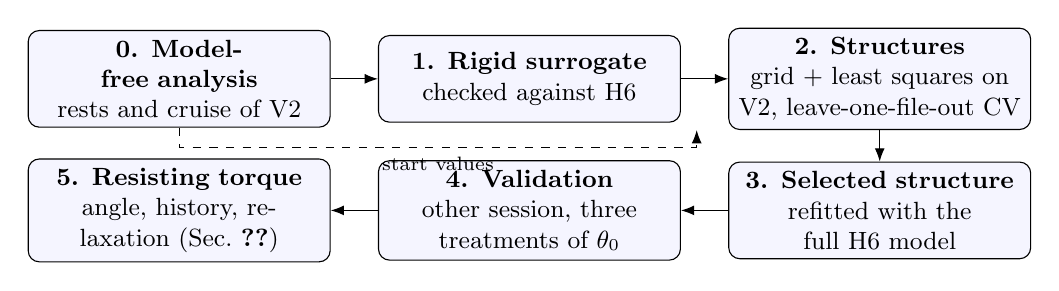
\begin{tikzpicture}[node distance=4mm and 6mm, every node/.style={font=\small},
  box/.style={draw, rounded corners, align=center, text width=3.6cm, minimum height=1.1cm, fill=blue!4}]
\node[box] (a) {\textbf{0. Model-free analysis}\\ rests and cruise of V2};
\node[box, right=of a] (b) {\textbf{1. Rigid surrogate}\\ checked against H6};
\node[box, right=of b] (c) {\textbf{2. Structures}\\ grid + least squares on V2, leave-one-file-out CV};
\node[box, below=of c] (d) {\textbf{3. Selected structure}\\ refitted with the full H6 model};
\node[box, left=of d] (e) {\textbf{4. Validation}\\ other session, three treatments of $\theta_0$};
\node[box, left=of e] (f) {\textbf{5. Resisting torque}\\ angle, history, relaxation (Sec.~\ref{sec:cables})};
\draw[-{Latex}] (a) -- (b); \draw[-{Latex}] (b) -- (c); \draw[-{Latex}] (c) -- (d); \draw[-{Latex}] (d) -- (e); \draw[-{Latex}] (e) -- (f);
\draw[-{Latex}, dashed] (a.south) |- ++(0,-0.25) -| ([xshift=-4mm]c.south west) node[pos=0.25, below, font=\scriptsize]{start values};
\end{tikzpicture}
\caption{Flow of the work. Steps 0--4 are in \texttt{v2\_identification.py}, step 5 in \texttt{cable\_torque\_analysis.py}.}\label{fig:flow}
\end{figure}

\subsection{Step 0: model-free analysis}\label{sec:modelfree}
Before any simulation, two regressions on the measured torque $K_t i$ of the V2 files give the order of magnitude of the friction and of the position-dependent torque, and the start values of the fits.
\begin{itemize}
\item \textbf{Cruise at 10\,deg/s.} In the cruise the acceleration is zero, so the motor torque equals the resisting torque. Over the cruise samples of both directions $d=\pm1$,
\begin{equation}
K_t i = F\,d + K\theta + c ,\label{eq:cruise}
\end{equation}
where $F$ is the friction at 10\,deg/s and $K\theta+c$ the position-dependent torque. At the same angle, the half-sum of the torques of the two directions is the position-dependent torque and the half-difference is the friction.
\item \textbf{Rests} (from 3\,s after a move to the next move): the holding torque regressed on the angle and on the direction $d$ of the last move, $K_t i = K\theta+c+h\,d$.
\end{itemize}
Results (Table~\ref{tab:modelfree}, Figure~\ref{fig:modelfree}):
\begin{itemize}
\item the friction at 10\,deg/s is \FAz\,N\,m in azimuth and \FEl\,N\,m in elevation;
\item in the cruise, the position-dependent torque looked negligible in azimuth (gradient \KcrAz\,N\,m/rad) and clear in elevation (\KcrEl\,N\,m/rad). Here the cruise is selected by the \emph{command} speed: the encoder lags the command by about $v/K_{pp}\approx1.5^\circ$, so the first degrees after a start still carry acceleration torque (the bump between 0 and $+2^\circ$ of Figure~\ref{fig:modelfree}), and in azimuth the 8--10\,Hz oscillation of the loop adds noise. Section~\ref{sec:angle} repeats the analysis selecting by the \emph{encoder} speed: the azimuth has a position-dependent torque as well (\KencAz\,N\,m/rad), and the friction at 10\,deg/s is \FencAz\ and \FencEl\,N\,m. The values of this step were used only as start values;
\item at rest the holding torque depends above all on the direction of the last move ($h$ = \HrestAz\ and \HrestEl\,N\,m): the friction stays loaded at its sliding level when the axis stops;
\item in the rests of a doublet, angle and direction go together (the positive angles are always reached with a positive move), so the rest gradients (\KrestAz\ and \KrestEl\,N\,m/rad) mix the two effects. The cruise, which crosses the same angles in both directions, separates them.
\end{itemize}
This explains why the cable spring of the earlier iteration I9a, fitted on 1$^\circ$ steps, came out at 12--16\,N\,m/rad: on those steps the angle and the direction of the last move coincide, and $K_c$ took up the memory of the friction.

\begin{table}[H]\centering\small
\caption{Model-free analysis of V2. Cruise: regression~\eqref{eq:cruise}, rms of its residual (the azimuth current carries an 8--10\,Hz oscillation of the loop). Rests: direction term $h$, gradient and rms.}\label{tab:modelfree}
\begin{tabular}{lrrrrrrr}\toprule
& \multicolumn{4}{c}{cruise at 10\,deg/s} & \multicolumn{3}{c}{rests} \\ \cmidrule(lr){2-5}\cmidrule(lr){6-8}
axis & $F$ [N\,m] & $K$ [N\,m/rad] & $c$ [N\,m] & rms [N\,m] & $h$ [N\,m] & $K$ [N\,m/rad] & rms [N\,m] \\ \midrule
azimuth & 0.374 & 0.16 & +0.049 & 0.51 & 0.201 & 1.12 & 0.10 \\
elevation & 0.384 & 1.29 & +0.074 & 0.11 & 0.305 & 1.62 & 0.15
\\ \bottomrule
\end{tabular}\end{table}
\begin{figure}[H]\centering
\includegraphics[width=0.95\linewidth]{figures/model_free.pdf}
\caption{Model-free analysis of V2. Top: holding torque $K_t i$ [N\,m] in the rests against the encoder angle [deg], by direction of the last move (bar: torque at the start and at the end of the rest), with the regression lines. Bottom: torque [N\,m] in the cruise at 10\,deg/s against the angle [deg]: samples, means per 2$^\circ$ bin and direction, half-sum (position-dependent torque) and half-difference (friction).}\label{fig:modelfree}
\end{figure}

\subsection{Goodness measure and cost}
\paragraph{Fit of a move.} For the encoder position $y$ of the moving axis in window $w$ (change from the window start) and the simulated $\hat y$,
\begin{equation}
\mathbf r_w=\frac{\hat{\mathbf y}-\mathbf y}{\lVert\mathbf y-\bar y\rVert},\qquad e_w=\lVert\mathbf r_w\rVert,\qquad \mathrm{fit}_w=100\,(1-e_w)\ \%,
\end{equation}
the NRMSE fit of the System Identification Toolbox. Every move weighs the same, whatever its amplitude.

\paragraph{Robust cost.} In a simulation driven by the measured current, a small error of the torque balance after a move integrates into a drift: some moves (mostly of 0.1--0.2$^\circ$, where the holding torque is close to the friction) reach fits of several hundred per cent below zero, and in plain least squares a single such move would steer the whole estimate. The cost is therefore
\begin{equation}
J=\sum_w \rho(e_w^2),\qquad \rho(z)=c^2\ln\!\bigl(1+z/c^2\bigr),\quad c=1 ,
\end{equation}
a Cauchy loss of the error of each move: equal to least squares for good moves ($e_w\ll1$, fit near 100\,\%), it grows only logarithmically for moves whose fit is below about 0\,\%. It is implemented by scaling each $\mathbf r_w$ by $\sqrt{\rho(e_w^2)}/e_w$. The moves the model loses still count in the cross-validation scores.

\paragraph{Parameters.} The positive parameters are fitted on their logarithm (relative steps, positivity), $\theta_0$ on its value. Bounds: $\kappa_i\in[0.5,2]$, $\sigma_0\in[50,10^5]$\,N\,m/rad, $T_c\in[0.01,3]$\,N\,m, $T_s/T_c\in[1,10]$, $v_s\in[10^{-4},0.1]$\,rad/s, $b\in[10^{-4},10]$\,N\,m\,s/rad, $K_c\in[10^{-3},50]$\,N\,m/rad, $\theta_0\in[-30,30]^\circ$.

\subsection{Start values and least squares}
\begin{itemize}
\item \textbf{Grid.} The first structures of each axis start from the best point of a grid on the cost: $\kappa_i\in\{0.85,1,1.15\}$, $T_c\in\{0.6,0.85,1.1\}\times F$, $T_s/T_c\in\{1.1,1.5,2.5\}$ and, with the cable spring, $K_c\in\{0.3,1,3\}\times K$ and $\theta_0\in\{-5,0,+5\}^\circ$ around the value of the cruise (27 or 243 points). $\sigma_0$ and $v_s$ start from their nominal values (below), $b$ from 0.02\,N\,m\,s/rad. The other structures start from the fit of the structure they derive from.
\item \textbf{Least squares.} Trust-region reflective (\texttt{scipy.optimize.least\_squares}), Jacobian by finite differences with a 3\,\% step on the logarithm, at most 40 evaluations of the cost.
\end{itemize}

\subsection{Choice of the structure: leave-one-file-out cross-validation}
\paragraph{Why.} The earlier iterations showed that a parameter the data do not determine still improves the fit on the identification moves, but degrades the prediction of new moves (overfitting). The structure is therefore chosen on the moves it was \emph{not} fitted on.
\paragraph{Folds.} One V2 file out at a time (7 folds in azimuth, 8 in elevation). The structure is refitted on the other files, starting from its fit on all of V2 (at most 12 evaluations), and the moves of the file left out are simulated with the refitted parameters. The cross-validation (CV) score of a structure is the median of the fits of all the held-out moves; the worst one and the mean of $(1-\mathrm{fit})^2$ are also reported.
\paragraph{Structures compared,} for each axis, in three steps:
\begin{enumerate}
\item cable spring or not, all the friction parameters fitted;
\item from the better of the two, each of $\sigma_0$, $v_s$ (and $b$ in elevation) \emph{fixed} instead of fitted, at its nominal value times $1/3$, 1 and 3 ($b$ only at 0). Nominal values: $\sigma_0$ of the H6 Dahl element tuned on the frequency responses (\nominalSigmaAz\ and \nominalSigmaEl\,N\,m/rad), $v_s=0.005$\,rad/s (no independent measurement: the factors show whether the choice matters), $b=0$ (H6). A fixing is accepted when its best variant scores within 1 point of step 1;
\item the accepted fixings together.
\end{enumerate}
\paragraph{Rule,} set before the run: the structure with the best CV median; among those within 1 point of it, the one with the fewest free parameters (then the better median).

\subsection{Final fit and uncertainty}
The selected structure is refitted with the \emph{full} H6 model on all of V2, starting from its surrogate fit (at most 8 evaluations). Two measures of the uncertainty of the parameters:
\begin{itemize}
\item \textbf{Jacobian}: $\mathrm{cov}=s^2\,(\mathbf J^T\mathbf J\,n_\mathrm{eff}/N)^{-1}$, with $s^2=\sum r^2/(n_\mathrm{eff}-p)$ and $n_\mathrm{eff}$ the number of independent samples of the residuals (from their autocorrelation);
\item \textbf{jackknife} over the leave-one-file-out fits: $\sqrt{(n-1)/n\sum_k(p_k-\bar p)^2}$. The folds start from the fit on all of V2, so this measure is optimistic, while the Jacobian one is pessimistic where the cost is flat or rough.
\end{itemize}

\subsection{Validation protocol}
The parameters identified on V2 simulate the 26 moves of the other session with the full model. The neutral angle $\theta_0$ is treated in three ways, from the strictest:
\begin{enumerate}
\item $\theta_0$ of V2 (nothing estimated on the other session);
\item $\theta_0$ of the session: estimated alone on one file of the other session and used on the moves of the other three files; every file in turn;
\item $\theta_0$ of each file, estimated on the moves it is then scored on (an unknown initial condition, as \texttt{compare(\dots,'InitialCondition','estimate')} of the System Identification Toolbox).
\end{enumerate}

%% ===================================================================================================
\section{Results of the identification}\label{sec:results}
\subsection{Structures}
Table~\ref{tab:structures} and Figure~\ref{fig:cv} give all the structures compared.
\begin{itemize}
\item \textbf{Cable spring.} It is needed in elevation (CV median from \cvNoSpringEl\ to \cvSpringEl\,\%) and it helps in azimuth (from \cvNoSpringAz\ to \cvSpringAz\,\%).
\item \textbf{No overfitting.} For every structure with the cable spring the CV median stays within \cvGapAz\ (azimuth) and \cvGapEl\ (elevation) points of the identification median: the parameters fitted on part of V2 predict the rest equally well. Without the spring the elevation loses \cvGapNoSpringEl\ points in cross-validation: the friction parameters then try to imitate the missing position torque, differently in every fold. With the earlier I9a parameters, fitted on the 1$^\circ$ steps, the median fit on V2 was $-39$\,\% in azimuth and $-2.5$\,\% in elevation.
\item \textbf{Fixed parameters.}
  \begin{itemize}
  \item In azimuth $\sigma_0$ fixed at 3 times the nominal value gives the best CV median, \cvSelAz\,\%.
  \item In elevation $v_s$ fixed at 3 times the nominal value gives \cvSelEl\,\%.
  \item Fixing $\sigma_0$, $v_s$ and $b$ together in elevation costs 1.5 points and is not selected.
  \item The scores of the variants are not monotonic in the factor (for example, $\sigma_0$ at 1, 1/3 and 3 times the nominal value in azimuth), so differences of one or two points come from the roughness of the cost as much as from the structure.
  \end{itemize}
\item \textbf{Selected:} azimuth: \selAz; elevation: \selEl.
\end{itemize}
\begin{table}[H]\centering\small
\caption{Structures compared (selected in bold): free parameters, median fit on all of V2 (identification), median, worst and mean $(1-\mathrm{fit})^2$ of the held-out moves (cross-validation), rigid surrogate.}\label{tab:structures}
\begin{tabular}{llrrrrr}\toprule
axis & structure & free & ident. [\%] & CV median [\%] & CV worst [\%] & CV $\overline{(1-\mathrm{fit})^2}$ \\ \midrule
azimuth & no cable spring, all free & 5 & 81.5 & 81.1 & -97 & 0.24 \\
azimuth & cable spring, all free & 7 & 89.0 & 88.8 & -37 & 0.22 \\
azimuth & cable spring, $\sigma_0$ fixed $\times\frac13$ & 6 & 88.5 & 88.5 & -46 & 0.22 \\
azimuth & cable spring, $\sigma_0$ fixed $\times1$ & 6 & 81.6 & 81.6 & -5 & 0.15 \\
azimuth & \textbf{cable spring, $\sigma_0$ fixed $\times3$} & 6 & 89.5 & 89.5 & -23 & 0.12 \\
azimuth & cable spring, $v_s$ fixed $\times\frac13$ & 6 & 84.4 & 84.5 & -144 & 0.40 \\
azimuth & cable spring, $v_s$ fixed $\times1$ & 6 & 82.9 & 82.9 & -102 & 0.26 \\
azimuth & cable spring, $v_s$ fixed $\times3$ & 6 & 88.5 & 86.2 & -19 & 0.18 \\
\midrule
elevation & no cable spring, all free & 6 & 52.5 & 36.5 & -879 & 4.81 \\
elevation & cable spring, all free & 8 & 82.9 & 84.1 & -354 & 1.36 \\
elevation & cable spring, $\sigma_0$ fixed $\times\frac13$ & 7 & 85.9 & 86.3 & 5 & 0.14 \\
elevation & cable spring, $\sigma_0$ fixed $\times1$ & 7 & 81.8 & 79.6 & -16 & 0.14 \\
elevation & cable spring, $\sigma_0$ fixed $\times3$ & 7 & 82.5 & 82.5 & -25 & 0.21 \\
elevation & cable spring, $v_s$ fixed $\times\frac13$ & 7 & 84.2 & 85.8 & -159 & 0.47 \\
elevation & cable spring, $v_s$ fixed $\times1$ & 7 & 87.5 & 86.4 & -161 & 0.47 \\
elevation & \textbf{cable spring, $v_s$ fixed $\times3$} & 7 & 87.4 & 86.9 & -348 & 1.33 \\
elevation & cable spring, $b_{\theta,h}$ fixed 0 & 7 & 85.6 & 85.5 & -187 & 0.61 \\
elevation & cable spring, $\sigma_0$, $v_s$, $b_{\theta,h}$ fixed & 5 & 85.1 & 85.4 & -391 & 1.05
\\ \bottomrule
\end{tabular}\end{table}
\begin{figure}[H]\centering
\includegraphics[width=\linewidth]{figures/cross_validation.pdf}
\caption{Cross-validation of the structures: CV median of the held-out moves (bars, green the selected one) and median fit on all of V2 (diamonds), NRMSE fit of the encoder position [\%].}\label{fig:cv}
\end{figure}

\subsection{Parameters}
\begin{table}[H]\centering\small
\caption{Parameters of the selected structures, full H6 model: value, fitted or fixed, standard error from the Jacobian (relative for the positive parameters, absolute for $\theta_0$) and jackknife over the cross-validation folds.}\label{tab:params}
\begin{tabular}{lllrlrr}\toprule
axis & parameter & unit & value & & s.e. Jacobian & s.e. jackknife \\ \midrule
azimuth & $\kappa_i$ & -- & 0.9644 & fitted & 30\,\% & 4\,\% \\
azimuth & $T_c$ & N\,m & 0.2316 & fitted & 34\,\% & 12\,\% \\
azimuth & $T_s/T_c$ & -- & 7.934 & fitted & 348\,\% & 11\,\% \\
azimuth & $v_s$ & rad/s & 0.005816 & fitted & 116\,\% & 37\,\% \\
azimuth & $\sigma_0$ & N\,m/rad & 4513 & fixed & -- & -- \\
azimuth & $K_c$ & N\,m/rad & 0.9279 & fitted & 264\,\% & 20\,\% \\
azimuth & $\theta_0$ & deg & -2.678 & fitted & 12$^\circ$ & 1.4$^\circ$ \\
\midrule
elevation & $\kappa_i$ & -- & 1.071 & fitted & 38\,\% & 5\,\% \\
elevation & $T_c$ & N\,m & 0.4073 & fitted & 10\,\% & 6\,\% \\
elevation & $T_s/T_c$ & -- & 1.139 & fitted & 151\,\% & 8\,\% \\
elevation & $v_s$ & rad/s & 0.015 & fixed & -- & -- \\
elevation & $\sigma_0$ & N\,m/rad & 1703 & fitted & 330\,\% & 97\,\% \\
elevation & $b_{\theta,h}$ & N\,m\,s/rad & 0.0004712 & fitted & $>10^4$\,\% & 159\,\% \\
elevation & $K_c$ & N\,m/rad & 1.661 & fitted & 83\,\% & 14\,\% \\
elevation & $\theta_0$ & deg & -2.156 & fitted & 3.2$^\circ$ & 0.59$^\circ$
\\ \bottomrule
\end{tabular}\end{table}
Reading of Table~\ref{tab:params}:
\begin{itemize}
\item \textbf{Torque scale $\kappa_i$} \scaleAz\ and \scaleEl: the measured current and $K_t$ are consistent with the CAD inertia within a few per cent.
\item \textbf{Friction.}
  \begin{itemize}
  \item Sliding level $T_c$ = \TcAz\,N\,m (azimuth) and \TcEl\,N\,m (elevation).
  \item Viscous term of the elevation: it goes to its lower bound ($b$ = \bEl\,N\,m\,s/rad). With moves at different speeds, the friction at 10\,deg/s turns out to be all Coulomb.
  \item The elevation breaks away at $T_s$ = \TsEl\,N\,m ($T_s/T_c$ = \TsRatioEl), as the 0.1$^\circ$ moves show directly.
  \item In azimuth $T_s/T_c$ = \TsRatioAz\ acts only below $v_s$ = \vsDegAz\,deg/s. $T_s$ and $v_s$ work as a pair (their product shapes the start of the motion) and must not be read as a break-away torque.
  \end{itemize}
\item \textbf{Cable spring.}
  \begin{itemize}
  \item Elevation: $K_c$ = \KcEl\,N\,m/rad and $\theta_0$ = \thzEl$^\circ$, consistent with the cruise (Section~\ref{sec:modelfree}).
  \item Azimuth: $K_c$ = \KcAz\,N\,m/rad, of the same order as the gradient of the cruise selected by the encoder speed (\KencAz\,N\,m/rad, Section~\ref{sec:angle}); $\theta_0$ is poorly determined because the torque is small.
  \end{itemize}
\item \textbf{Uncertainty.}
  \begin{itemize}
  \item The two measures disagree. The jackknife says that the best-determined parameters are $\kappa_i$, $T_c$, $T_s/T_c$ and the elevation $K_c$ and $\theta_0$ (a few to 15\,\%, 0.6$^\circ$).
  \item The poorly determined ones are $\sigma_0$ of the elevation, $v_s$ of the azimuth and $b$, which sits at its bound.
  \item The large Jacobian errors come from flat directions of the cost (for example $T_s$ against $v_s$). The predictions do not depend on them: the CV scores stay close to the identification ones.
  \end{itemize}
\end{itemize}

\subsection{Position fit}
\begin{table}[H]\centering\small
\caption{NRMSE fit of the encoder position [\%], full H6 model: median [min, max] and number of moves. The validation moves are counted once per calibration file in the ``one other file'' line.}\label{tab:fits}
\begin{tabular}{lrlrl}\toprule
& \multicolumn{2}{c}{azimuth} & \multicolumn{2}{c}{elevation} \\ \cmidrule(lr){2-3}\cmidrule(lr){4-5}
set & moves & fit & moves & fit \\ \midrule
identification, V2 (49 moves) & 25 & 89.6 [-3, 97] & 24 & 87.8 [27, 96] \\
validation, $\theta_0$ of V2 & 12 & 85.6 [67, 98] & 14 & 49.7 [-83, 59] \\
validation, $\theta_0$ of the session from one other file & 36 & 89.5 [76, 97] & 42 & 85.4 [77, 94] \\
validation, $\theta_0$ of each file & 12 & 90.2 [86, 93] & 14 & 86.4 [78, 94]
\\ \bottomrule
\end{tabular}\end{table}
\begin{itemize}
\item \textbf{Identification (V2):} \fitIdAz\,\% (azimuth) and \fitIdEl\,\% (elevation) in median.
\item \textbf{Validation with $\theta_0$ of V2:} \fitValAz\ and \fitValEl\,\%. In elevation the positive moves stop short and the negative ones run on (Figure~\ref{fig:posval}): a constant torque is missing.
\item \textbf{With $\theta_0$ of the session} (estimated on one file, used on the other three): \fitValSesAz\ and \fitValSesEl\,\%, almost the same as with $\theta_0$ of each file (\fitValSeqAz\ and \fitValSeqEl\,\%). The missing torque is a property of the session, not of the single file.
\item \textbf{Adequacy (90\,\%):} reached only by the azimuth, and only with $\theta_0$ of each file.
\item \textbf{By amplitude} (Table~\ref{tab:fitclasses}, Figure~\ref{fig:fitamp}):
  \begin{itemize}
  \item the moves from 1 to 10$^\circ$ are reproduced at about 90\,\% in median;
  \item the moves of 0.1--0.5$^\circ$, decided by the pre-sliding and the break-away, are the worst and the most scattered;
  \item the longest moves (13--30$^\circ$) lose a few points to the drift in the cruise: in an open-loop simulation a small error of the torque balance integrates twice over 1.5--3\,s.
  \end{itemize}
\end{itemize}
\begin{table}[H]\centering\small
\caption{Identification fit [\%] by amplitude of the move, full H6 model: number of moves and median [min, max].}\label{tab:fitclasses}
\begin{tabular}{lrlrl}\toprule
& \multicolumn{2}{c}{azimuth} & \multicolumn{2}{c}{elevation} \\ \cmidrule(lr){2-3}\cmidrule(lr){4-5}
amplitude [deg] & moves & fit & moves & fit \\ \midrule
0.1--0.5 & 5 & 52.3 [-3, 95] & 5 & 68.5 [27, 90] \\
1--10 & 12 & 90.7 [82, 97] & 14 & 88.2 [75, 96] \\
13--30 & 8 & 86.8 [78, 95] & 5 & 90.2 [80, 96]
\\ \bottomrule
\end{tabular}\end{table}
\begin{figure}[H]\centering
\includegraphics[width=\linewidth]{figures/fit_vs_amplitude.pdf}
\caption{Fit of each move [\%] against its amplitude [deg], selected structure: identification on V2 (full model), cross-validation (held-out V2 moves, rigid surrogate), validation on the other session with $\theta_0$ of V2 (full model). Fits below $-100$\,\% are drawn at $-100$\,\%.}\label{fig:fitamp}
\end{figure}
\begin{figure}[H]\centering
\includegraphics[width=0.82\linewidth]{figures/position_identification.pdf}
\caption{Identification: change of the encoder position [mdeg or deg] in the window, measured and simulated (full model), for the smallest, a middle and the largest move of each axis.}\label{fig:posid}
\end{figure}
\begin{figure}[H]\centering
\includegraphics[width=0.82\linewidth]{figures/position_validation.pdf}
\caption{Validation on the other session with $\theta_0$ of V2: change of the encoder position [mdeg] in the window, measured and simulated (full model).}\label{fig:posval}
\end{figure}

%% ===================================================================================================
\section{Resisting torque: angle, history and the cables}\label{sec:cables}
\paragraph{Questions.} Does the resisting torque change with the angle? After a doublet, back at 0, is the resisting torque different from before? A large, non-repeatable change would be the symptom of a cable torque that cannot be modelled.

\paragraph{How it is measured.} The resisting torque is what the motor has to supply when the axis does not accelerate, so it can be read from the measured $K_t i$ without any model in two situations:
\begin{itemize}
\item \textbf{cruise} at constant speed: friction plus position-dependent torque;
\item \textbf{rest} at constant position: holding torque, that is position-dependent torque plus the friction left loaded at the stop.
\end{itemize}
The analysis is in \texttt{cable\_torque\_analysis.py}; it uses all sixteen V2 files in the order they were recorded (Table~\ref{tab:session}).

\subsection{Does the resisting torque change with the angle?}\label{sec:angle}
\paragraph{Method.} The cruise is now selected by the \emph{encoder} speed (low-passed at 20\,Hz, within 3\,\% of 10\,deg/s), which leaves out the acceleration of the axis behind the command. For every file, and for all the files together, the regression~\eqref{eq:cruise} separates the friction $F$ from the position-dependent torque $K\theta+c$. At each angle, the half-sum of the two directions is the position-dependent torque and the half-difference the friction. A file enters only when its two directions cross at least three common 1$^\circ$ bins.

\paragraph{Results} (Figure~\ref{fig:cruisefiles}, Table~\ref{tab:cruisefiles}).
\begin{itemize}
\item \textbf{Position-dependent torque: yes, in both axes.}
  \begin{itemize}
  \item It is close to linear, \KencAz\,N\,m/rad in azimuth and \KencEl\,N\,m/rad in elevation over all files: about $\pm0.3$\,N\,m over $\pm12^\circ$, the same order as the friction.
  \item In elevation the four files that reach a cruise (doublets of 5, 8, 10 and 15$^\circ$) give the same curve within a few hundredths of a N\,m: within the session the torque is a repeatable function of the angle.
  \item In azimuth the 8$^\circ$ file overlaps the sweep where both exist.
  \item The azimuth axis is vertical, so gravity cannot produce this torque: the cables (cable wrap) are the natural candidate. In elevation cables and a residual imbalance would both give it, and over $\pm15^\circ$ the two cannot be told apart.
  \end{itemize}
\item \textbf{Friction at 10\,deg/s.}
  \begin{itemize}
  \item Elevation: almost independent of the angle, \FencEl\,N\,m (\FspreadEl\ from file to file), slightly higher above $+8^\circ$.
  \item Azimuth: it changes with the angle, from about 0.4\,N\,m at $-10^\circ$ to 0.2--0.27\,N\,m between $+5$ and $+10^\circ$. Only the sweep file covers this range, so the repeatability of this trend is not tested. The model has a constant $T_c$.
  \end{itemize}
\end{itemize}
\begin{figure}[H]\centering
\includegraphics[width=0.95\linewidth]{figures/cruise_per_file.pdf}
\caption{Cruise at 10\,deg/s selected by the encoder speed, file by file, means per 1$^\circ$ bin. Top: position-dependent torque (half-sum of the two directions) [N\,m] against the encoder angle [deg]. Bottom: friction (half-difference) [N\,m].}\label{fig:cruisefiles}
\end{figure}
\begin{table}[H]\centering\small
\caption{Cruise regression $K_ti=F\,d+K\theta+c$, encoder-speed selection, file by file and all files together; neutral angle $-c/K$ of the position torque.}\label{tab:cruisefiles}
\begin{tabular}{llrrrr}\toprule
axis & file & $F$ [N\,m] & $K$ [N\,m/rad] & $c$ [N\,m] & $-c/K$ [deg] \\ \midrule
azimuth & azimut\_1deg\_15deg & 0.282 & 1.26 & +0.036 & -1.6 \\
azimuth & azimut\_8deg\_minus8deg & 0.359 & 2.80 & +0.082 & -1.7 \\
elevation & elevation\_5deg\_minus5deg & 0.339 & 1.78 & +0.074 & -2.4 \\
elevation & elevation\_8deg\_minus8deg & 0.328 & 1.27 & +0.037 & -1.6 \\
elevation & elevation\_10deg\_minus10deg & 0.343 & 1.26 & +0.045 & -2.0 \\
elevation & elevation\_15deg\_minus15deg & 0.375 & 1.40 & +0.064 & -2.6 \\
azimuth & \textbf{all files} & 0.286 & 1.31 & +0.033 & -1.4 \\
elevation & \textbf{all files} & 0.355 & 1.38 & +0.059 & -2.4
\\ \bottomrule
\end{tabular}\end{table}

\subsection{Holding torque and the amplitude of the last move}\label{sec:holding}
\paragraph{Method.} The holding torque 3\,s after each move, multiplied by the sign of the move, against the amplitude of the move. In elevation the position-dependent torque of the cruise is subtracted.
\paragraph{Results} (Figure~\ref{fig:holding}).
\begin{itemize}
\item In a Dahl element the friction left loaded at the stop is the sliding level after any move longer than a few $g/\sigma_0$ (3--14\,mdeg here): it should not depend on the amplitude.
\item \textbf{Azimuth:} the holding torque grows from 0.1--0.2\,N\,m after moves of 0.1--2$^\circ$ to 0.35--0.45\,N\,m after moves of 5$^\circ$ or more, and levels off there.
\item \textbf{Elevation:} the same trend, weaker: 0.37--0.44\,N\,m after moves of 1--3$^\circ$, 0.45--0.54\,N\,m after 5$^\circ$ or more.
\item The resisting torque therefore has a second, slow hysteretic part, whose transition spreads over several degrees instead of a few millidegrees. It is the behaviour of a flexible element with internal friction (a cable bundle bending and its conductors sliding on each other), and of a multi-element (Maxwell-slip) friction model, not of a single Dahl element.
\item The elevation moves of 0.5$^\circ$ are an exception: the axis overshoots by 2--3\,mdeg and the loop pulls it back, and this small reversal unloads the friction (holding torque close to zero).
\end{itemize}
\begin{figure}[H]\centering
\includegraphics[width=\linewidth]{figures/holding_vs_amplitude.pdf}
\caption{Holding torque 3\,s after a move, times the sign of the move [N\,m], against the amplitude of the move [deg]; squares: rests at $\pm A$, circles: rests at 0; dashed: friction at 10\,deg/s of the command-speed cruise. Elevation: position-dependent torque of the cruise removed.}\label{fig:holding}
\end{figure}

\subsection{Back at 0 after a doublet}\label{sec:return}
\paragraph{Method.} Every doublet starts and ends at 0, and the last move of a doublet ($-A\to0$) is positive, like the last move before the next file. Between files the axis is not moved. The holding torque at 0 can thus be compared at three times: before the doublet (start of the file), 3\,s after its end, and about one minute later (start of the next file). Figure~\ref{fig:timeline} shows the whole session; Table~\ref{tab:return0} gives the values.
\paragraph{Elevation.}
\begin{itemize}
\item Before the doublets: 0.36--0.41\,N\,m.
\item 3\,s after: 0.47--0.54\,N\,m after the doublets of 1--15$^\circ$, that is 0.08--0.18\,N\,m more, growing with the amplitude (Section~\ref{sec:holding}).
\item Within about one minute the torque relaxes back to 0.36--0.41\,N\,m, the value before the doublet (start of the next file).
\item Across the 15 minutes of the elevation session, with excursions growing from $\pm0.1$ to $\pm15^\circ$, the torque at 0 before each doublet does not drift.
\item The exception is the 0.5$^\circ$ doublet, which leaves the torque close to zero for the reason given in Section~\ref{sec:holding}; the next (1$^\circ$) doublet brings it back.
\end{itemize}
\paragraph{Azimuth.}
\begin{itemize}
\item The torque at 0 after a doublet depends on its amplitude: 0.17--0.19\,N\,m after the doublets of 0.1--1$^\circ$, 0.36--0.38\,N\,m after those of 3--15$^\circ$.
\item It relaxes little (Section~\ref{sec:relax}), so the next file starts almost at the same value: 0.31--0.33\,N\,m after the 3 and 8$^\circ$ doublets, 0.18\,N\,m after the 0.1 and 1$^\circ$ ones.
\item The change is reversible: after the 8$^\circ$ doublet (0.33\,N\,m) a 0.1$^\circ$ doublet brings it back to 0.18\,N\,m. The torque at 0 remembers the amplitude of the last excursion; it does not accumulate.
\item The 1$^\circ$ file starts at $-0.10$\,N\,m after a pause of 19\,min since the previous file, whose history is unknown.
\end{itemize}
\begin{figure}[H]\centering
\includegraphics[width=\linewidth]{figures/session_timeline.pdf}
\caption{V2 session in recording order (time from the file modification times) [min]. For each axis: motor torque $K_ti$ [N\,m] (every 50th sample) with the start of each rest at 0$^\circ$ (red) and at $\pm A$ (orange), and the encoder angle [deg] with the name of the file.}\label{fig:timeline}
\end{figure}
\begin{table}[H]\centering\scriptsize
\caption{Holding torque at 0$^\circ$ in recording order: time in the session [min], before the doublet (start of the file) or after it (3\,s after the last move), last move [deg], length of the rest [s], torque at the start and at the end of the rest [N\,m].}\label{tab:return0}
\begin{tabular}{lllllrrr}\toprule
axis & file & time & rest & last move & length & start & end \\ \midrule
azimuth & azimut\_1deg\_15deg & 1.5 & after the doublet & +15.00 & 4 & +0.366 & +0.350 \\
azimuth & azimut\_1deg\_15deg\_v2 & 28.9 & after the doublet & +15.00 & 59 & +0.426 & +0.347 \\
azimuth & azimut\_1deg\_minus1deg & 47.2 & before the doublet & -- & 9 & -0.100 & -0.100 \\
azimuth & azimut\_1deg\_minus1deg & 48.6 & after the doublet & +1.00 & 14 & +0.194 & +0.187 \\
azimuth & azimut\_3deg\_minus3deg & 50.0 & before the doublet & -- & 4 & +0.181 & +0.181 \\
azimuth & azimut\_3deg\_minus3deg & 51.5 & after the doublet & +3.00 & 4 & +0.356 & +0.341 \\
azimuth & azimut\_5deg\_minus5deg & 52.2 & before the doublet & -- & 2 & +0.312 & +0.312 \\
azimuth & azimut\_5deg\_minus5deg & 53.6 & after the doublet & +5.00 & 8 & +0.356 & +0.337 \\
azimuth & azimut\_8deg\_minus8deg & 55.7 & after the doublet & +8.00 & 14 & +0.376 & +0.344 \\
azimuth & azimut\_01deg\_minus01deg & 56.7 & before the doublet & -- & 6 & +0.328 & +0.326 \\
azimuth & azimut\_01deg\_minus01deg & 57.9 & after the doublet & +0.10 & 18 & +0.183 & +0.181 \\
azimuth & azimut\_05deg\_minus05deg & 59.9 & before the doublet & -- & 6 & +0.180 & +0.180 \\
azimuth & azimut\_05deg\_minus05deg & 61.2 & after the doublet & +0.50 & 17 & +0.169 & +0.164 \\
\midrule
elevation & elevation\_01deg\_minus01deg & 64.1 & after the doublet & +0.10 & 14 & +0.393 & +0.353 \\
elevation & elevation\_05deg\_minus05deg & 64.8 & before the doublet & -- & 8 & +0.321 & +0.320 \\
elevation & elevation\_05deg\_minus05deg & 66.3 & after the doublet & +0.50 & 9 & +0.052 & -0.037 \\
elevation & elevation\_1deg\_minus1deg & 67.0 & before the doublet & -- & 3 & -0.020 & -0.019 \\
elevation & elevation\_1deg\_minus1deg & 68.3 & after the doublet & +1.00 & 17 & +0.471 & +0.435 \\
elevation & elevation\_3deg\_minus3deg & 69.3 & before the doublet & -- & 8 & +0.411 & +0.410 \\
elevation & elevation\_3deg\_minus3deg & 70.7 & after the doublet & +3.00 & 14 & +0.493 & +0.432 \\
elevation & elevation\_5deg\_minus5deg & 71.7 & before the doublet & -- & 5 & +0.359 & +0.357 \\
elevation & elevation\_5deg\_minus5deg & 73.0 & after the doublet & +5.00 & 19 & +0.517 & +0.441 \\
elevation & elevation\_8deg\_minus8deg & 74.0 & before the doublet & -- & 3 & +0.374 & +0.372 \\
elevation & elevation\_8deg\_minus8deg & 75.3 & after the doublet & +8.00 & 20 & +0.529 & +0.453 \\
elevation & elevation\_10deg\_minus10deg & 76.2 & before the doublet & -- & 6 & +0.387 & +0.386 \\
elevation & elevation\_10deg\_minus10deg & 77.6 & after the doublet & +10.00 & 14 & +0.532 & +0.455 \\
elevation & elevation\_15deg\_minus15deg & 78.6 & before the doublet & -- & 2 & +0.361 & +0.359 \\
elevation & elevation\_15deg\_minus15deg & 80.0 & after the doublet & +15.00 & 13 & +0.544 & +0.459
\\ \bottomrule
\end{tabular}\end{table}

\subsection{Relaxation at constant position}\label{sec:relax}
\paragraph{Observation} (Figure~\ref{fig:relax}, Table~\ref{tab:relax}).
\begin{itemize}
\item In the long rests the holding torque decays towards zero, while the encoder stays within one count (0.34\,mdeg).
\item Elevation: \relaxMedEl\,N\,m in median, up to \relaxMaxEl\,N\,m (\relaxRelEl\,\% of the torque), time constant about \tauEl\,s.
\item Azimuth: \relaxMedAz\,N\,m in median, up to \relaxMaxAz\,N\,m (\relaxRelAz\,\%), about \tauAz\,s.
\item With the pre-sliding stiffness of the model, 0.29\,N\,m would need a displacement of about 10\,mdeg, thirty times what is seen.
\end{itemize}
\paragraph{Two explanations.}
\begin{enumerate}
\item \textbf{The drive.} The velocity integrator keeps acting on a position error below one count against a bearing that is much stiffer at rest than $\sigma_0$ (at least $5\cdot10^4$\,N\,m/rad).
\item \textbf{The mechanism.} A stress relaxation of a viscoelastic element at constant position: the cable jackets or the seals.
\end{enumerate}
\paragraph{Test.} The change of torque that the integral action would give from the logged error, $K_tK_{pv}2\pi K_{iv}K_{pp}\int e\,dt$ (gains of I5), has the same sign as the observed change in \sameSignEl\,\% of the elevation rests and in \sameSignAz\,\% of the azimuth ones (Figure~\ref{fig:relaxint}).
\begin{itemize}
\item The test is not conclusive. In azimuth the logged error stays constant at 0.1--0.3\,mdeg for tens of seconds while the current hardly moves, which the integrator would not allow: the error seen by the drive is smaller than the logged one.
\item The logged data cannot decide between the two explanations. Logging the following error of the drive, or holding with the velocity integrator off, would.
\item Either way, the current model does not have it: the Dahl element keeps its torque at rest. The windows start from the measured holding torque, so this does not affect the identification, only long rests in a closed-loop simulation.
\end{itemize}
\begin{figure}[H]\centering
\includegraphics[width=\linewidth]{figures/relaxation.pdf}
\caption{Rests of 10\,s or more, coloured by the amplitude of the move before them [deg]. Top: change of the holding torque from 3\,s after the move [N\,m] against time [s]. Bottom: encoder minus command [mdeg] in the same rests.}\label{fig:relax}
\end{figure}
\begin{figure}[H]\centering
\includegraphics[width=\linewidth]{figures/relaxation_vs_integral_action.pdf}
\caption{Observed change of the holding torque over each rest [N\,m] against the change that the integral action of the drive would give from the logged position error [N\,m]; dashed: equality.}\label{fig:relaxint}
\end{figure}
\begin{table}[H]\centering\small
\caption{Relaxation in the rests of 10\,s or more after a move: number of rests, change of torque (median [largest]) [N\,m], relative change [\%], time constant of the exponential fit (median [min, max]) [s], change of the encoder (median [largest]) [mdeg], integral action from the logged error (median absolute) [N\,m], rests where the two have the same sign [\%].}\label{tab:relax}
\begin{tabular}{lrrrrrrr}\toprule
axis & rests & $|\Delta T|$ & rel. & $\tau$ & encoder & integral action & same sign \\ \midrule
azimuth & 18 & 0.028 [0.086] & 9 & 10 [2, 36] & 0.00 [0.15] & 0.079 & 44 \\
elevation & 23 & 0.099 [0.293] & 21 & 36 [1, 163] & 0.07 [2.68] & 0.164 & 91
\\ \bottomrule
\end{tabular}\end{table}

\subsection{From one session to the other}\label{sec:sessions}
\paragraph{Model-free.} On the rests after moves of 0.9$^\circ$ or more, with the gradient of the V2 cruise, $K_ti(3\,\mathrm s)-K\theta=c+h\,d$ gives the position-dependent torque at 0 ($c$) and the friction left at the stop ($h$) of each session (Table~\ref{tab:sessions}).
\begin{itemize}
\item \textbf{Elevation:} $c$ = \cSesVtwoEl\,N\,m in V2 and \cSesOtherEl\,N\,m in the other session, a shift of \cSesShiftEl\,N\,m. The friction left at the stop is the same in both sessions (\hSesVtwoEl\ and \hSesOtherEl\,N\,m).
\item \textbf{Azimuth:} no shift (\cSesShiftAz\,N\,m). The lower $h$ of the other session (\hSesOtherAz\ against \hSesVtwoAz\,N\,m) agrees with its moves being only 1--2$^\circ$ (Section~\ref{sec:holding}).
\end{itemize}
\paragraph{With the model.} $\theta_0$ fitted alone on each V2 file, all other parameters as identified (Figure~\ref{fig:theta0}, Table~\ref{tab:theta0}).
\begin{itemize}
\item \textbf{Elevation:} $\theta_0$ goes from \thzFileMinEl\ to \thzFileMaxEl$^\circ$ in V2 (standard deviation \thzFileSdEl$^\circ$), and from \thzOtherMinEl\ to \thzOtherMaxEl$^\circ$ in the other session. With $K_c$ = \KcEl\,N\,m/rad this is a shift of the position torque of \thzShiftTorqueEl\,N\,m at the same angle, the same as the model-free estimate.
\item \textbf{Azimuth:} $\theta_0$ is scattered (from \thzFileMinAz\ to \thzFileMaxAz$^\circ$, up to 0.12\,N\,m at $K_c$ = \KcAz\,N\,m/rad), but the extremes come from the 0.1 and 0.5$^\circ$ doublets and from the single move of \path{azimut_1deg_15deg_v2}, where $\theta_0$ is hardly determined. On the doublets of 1--8$^\circ$ and the sweep it stays between $-1.8$ and $0^\circ$ (0.03\,N\,m). The other session gives values in the same range.
\item Within a session the position torque is stable; between the two sessions (same day, about 7 hours apart) the elevation one moved by about 0.15\,N\,m.
\item The data cannot tell whether the cables settled in another layout, the balance of the telescope changed, or the zero of the encoder moved. A short calibration at the start of each session fixes it: with $\theta_0$ from one file, the other files of the session are predicted at \fitValSesEl\,\% (Table~\ref{tab:fits}).
\end{itemize}
\begin{table}[H]\centering\small
\caption{The two sessions on the rests: number of rests, position-dependent torque at 0 ($c$), friction left at the stop ($h$), rms of the regression [N\,m].}\label{tab:sessions}
\begin{tabular}{llrrrr}\toprule
axis & session & rests & $c$ [N\,m] & $h$ [N\,m] & rms [N\,m] \\ \midrule
azimuth & V2 & 22 & +0.018 & 0.237 & 0.098 \\
azimuth & other session & 6 & +0.000 & 0.177 & 0.029 \\
elevation & V2 & 19 & +0.105 & 0.427 & 0.097 \\
elevation & other session & 8 & -0.057 & 0.413 & 0.007
\\ \bottomrule
\end{tabular}\end{table}
\begin{figure}[H]\centering
\includegraphics[width=\linewidth]{figures/theta0_per_file.pdf}
\caption{Neutral angle $\theta_0$ [deg] of the position torque fitted file by file (V2, full model, other parameters as identified), its value on all of V2 (dashed), and the values of the four files of the other session.}\label{fig:theta0}
\end{figure}
\begin{table}[H]\centering\small
\caption{Neutral angle fitted file by file [deg] and median fit of the file [\%] with it and with $\theta_0$ of all of V2.}\label{tab:theta0}
\begin{tabular}{llrrr}\toprule
axis & file & $\theta_0$ [deg] & fit, own $\theta_0$ & fit, $\theta_0$ of V2 \\ \midrule
azimuth & azimut\_1deg\_15deg & -1.82 & 88.7 & 90.1 \\
azimuth & azimut\_1deg\_15deg\_v2 & -5.31 & 88.5 & 81.2 \\
azimuth & azimut\_1deg\_minus1deg & +0.00 & 94.0 & 82.5 \\
azimuth & azimut\_3deg\_minus3deg & -1.74 & 94.8 & 94.3 \\
azimuth & azimut\_5deg\_minus5deg & -1.68 & 91.1 & 89.6 \\
azimuth & azimut\_8deg\_minus8deg & -0.51 & 88.6 & 86.4 \\
azimuth & azimut\_01deg\_minus01deg & -7.50 & 37.8 & 26.2 \\
azimuth & azimut\_05deg\_minus05deg & -5.95 & 77.1 & 90.3 \\
azimuth & step\_1deg (other session) & +2.21 & -- & -- \\
azimuth & 1degAz\_zeroAz\_1degPol\_\_zeroPol (other session) & +0.00 & -- & -- \\
azimuth & 2degAz\_2degPol\_zeroAz\_zeroPol (other session) & -0.00 & -- & -- \\
azimuth & 2degPol\_zeroPol\_2degAz\_zeroAz (other session) & -0.51 & -- & -- \\
\midrule
elevation & elevation\_01deg\_minus01deg & -1.43 & 71.1 & 68.5 \\
elevation & elevation\_05deg\_minus05deg & -2.21 & 76.5 & 76.0 \\
elevation & elevation\_1deg\_minus1deg & -3.28 & 89.1 & 84.3 \\
elevation & elevation\_3deg\_minus3deg & -2.87 & 86.5 & 88.9 \\
elevation & elevation\_5deg\_minus5deg & -2.56 & 91.7 & 88.3 \\
elevation & elevation\_8deg\_minus8deg & -2.50 & 92.9 & 90.2 \\
elevation & elevation\_10deg\_minus10deg & -2.35 & 94.0 & 93.7 \\
elevation & elevation\_15deg\_minus15deg & -2.53 & 90.6 & 85.4 \\
elevation & step\_1deg (other session) & +2.28 & -- & -- \\
elevation & 1degAz\_zeroAz\_1degPol\_\_zeroPol (other session) & +2.16 & -- & -- \\
elevation & 2degAz\_2degPol\_zeroAz\_zeroPol (other session) & +2.86 & -- & -- \\
elevation & 2degPol\_zeroPol\_2degAz\_zeroAz (other session) & +2.57 & -- & --
\\ \bottomrule
\end{tabular}\end{table}

\subsection{Can the cables be modelled?}\label{sec:verdict}
Table~\ref{tab:verdict} collects the components of the resisting torque found in the data.
\begin{table}[H]\centering\small
\caption{Components of the resisting torque found in the V2 data.}\label{tab:verdict}
\begin{tabularx}{\linewidth}{L{3.2cm}L{2.6cm}L{2.6cm}L{2.2cm}Y}\toprule
component & size & repeatable in a session & in the current model & how to model it \\ \midrule
position-dependent torque & $\pm0.3$\,N\,m over $\pm12^\circ$, both axes & yes (elevation: same curve in four files) & yes, $K_c(\theta-\theta_0)$ & already in; a slow sweep would map its shape \\
friction at 10\,deg/s against the angle & elevation flat; azimuth 0.2--0.4\,N\,m & elevation yes; azimuth one file only & no (constant $T_c$) & $T_c(\theta)$, after a repeated sweep \\
holding torque growing with the last amplitude & up to 0.2\,N\,m & yes, and reversible & no & a second hysteretic element over degrees (Maxwell-slip, or a second Dahl element with $\sigma_0$ of a few N\,m/rad) \\
relaxation at rest & 0.03--0.29\,N\,m, $\tau$ 10--40\,s & yes & no & Maxwell (spring-damper) element, if mechanical; first decide whether it is the drive \\
offset between sessions & 0.15\,N\,m in elevation, none in azimuth & -- & calibrated $\theta_0$ & one calibration move per session \\ \bottomrule
\end{tabularx}\end{table}
\begin{itemize}
\item \textbf{No sign of erratic behaviour within a session.} After a doublet the torque at 0 changes by up to 0.15--0.2\,N\,m. The change depends on the amplitude of the last excursion and is reversible; in elevation it relaxes back within a minute. It is a deterministic hysteresis with a long memory, and a richer friction model can represent it.
\item \textbf{The part that cannot be predicted} from one session is the offset of the elevation position torque between sessions, about 0.15\,N\,m, comparable to 40\,\% of the friction. A calibration of one parameter on one short file of the session removes it.
\end{itemize}
\paragraph{Tests that would settle the open points.}
\begin{itemize}
\item A slow sweep (for example 1\,deg/s) over $\pm15^\circ$ in both directions, repeated twice, for each axis: the shape of the position torque and of the friction against the angle, and whether the azimuth friction trend repeats.
\item The doublets in decreasing amplitude, or a small doublet between two large ones: the memory of the amplitude seen in Section~\ref{sec:holding}.
\item Rests with the drive following error logged, or with the velocity integrator off: the origin of the relaxation.
\item A doublet at the start and at the end of each session: the drift of $\theta_0$ within a session and between sessions.
\end{itemize}


\end{document}
